\documentclass[presentation]{beamer}
\usepackage{will-beamer}
\usepackage[utf8]{inputenc}
\usepackage[T1]{fontenc}
\usepackage[english]{babel}
\usepackage{booktabs}
\usepackage{siunitx}
\tolerance=1000

\graphicspath{ 
  {figs/}, {towns-figs/}, {houston/}, {houston/figs/},
  {houston/turbfigs/}, {houston/globfigs/}, {oldtalks/}, {greece-figs/},
}

\setkeys{Gin}{width=\linewidth, height=0.85\textheight, keepaspectratio=true}

\title[\hii{} regions]{Structure and evolution of \hii{} regions:\\
  Reality, models, simulations}
\author{\textit{William J. Henney}}
\date[Cloudy 2016]{
  Cloudy: Emission Lines in Astrophysics
  \(\cdot\) August 2016 \(\cdot\) CDMX, Mexico
}

\institute[IRyA, UNAM, Mexico]
{
  \structure{Instituto de Radioastronomía y Astrofísica\\
    UNAM, Morelia, México}
}

\hypersetup{
  pdfkeywords={Massive Star Clusters, Astrophysics, Dynamics, Radiation},
  pdfsubject={},
  pdfcreator={Lovingly hand-crafted by the author using pdflatex and beamer}
}

\AtBeginSubsection[]
{
  \begin{frame}<beamer>
    \frametitle{Coming up \dots}
    \tableofcontents[
    currentsection, 
    currentsubsection, 
%    hideothersubsections
    ]
  \end{frame}
}

%\setbeamercolor{normal text}{fg=black!50!white,bg=blue!50!black}

\begin{document}

\maketitle

\tikzstyle{every picture}+=[remember picture, overlay]

\section{Introduction}

\subsection{Scope of the talk}


\begin{frame}
  \frametitle{What sort of regions are we talking about here?}
  \begin{block}{Photoionized nebulae, aka \hii{} regions}
    \begin{itemize}
    \item Around young(-ish) hot, high-mass stars
      \begin{itemize}
      \item Ages: \(10^5 \to 10^7\)~years (typically 1~million years)
      \item Spectral type: B\(0\) \(\to\) O\(3\) (typically O\(7\)V)
      \end{itemize}
    \item May be isolated \dots or in clusters of a few \dots or many
    \item Typically accompanied by a great number (hundreds, thousands,
      \dots)\\ of young, low-mass stars
    \end{itemize}
  \end{block}

  \begin{block}{Why are we interested?}
    \begin{enumerate}
    \item Massive stars \textit{clear out} and \textit{light up} their
      surroundings,\\ revealing outflows and disks around low-mass PMS
      stars:\\ proplyds, irradiated jets, etc
    \item Massive stars \textit{sculpt} their surroundings, directly
      influencing the star formation process: feedback, triggering, quenching
    \end{enumerate}
  \end{block}
  
\end{frame}

\subsection{Overview of physics}

\begin{frame}
  \frametitle{What makes \hii{} regions tick? (Classical view)}
  \begin{tikzpicture}
    \draw (current page.south west) node[above right, yshift=40pt, text width=0.6\textwidth]
    (strom spheres)
    {\includegraphics{strom-expansion}};
    %
    \draw (strom spheres.north) node[below=3pt, xshift=20pt, white, text
    width=0.4\textwidth]
    {
      Initial Strömgren sphere\\
      \(n_{\mathrm{i}} = n_{\mathrm{n}}\) \quad \(P_{\mathrm{i}} \gg P_{\mathrm{n}}\)
    };
    \draw (strom spheres.south) node[above=3pt, xshift=-30pt, white, text
    width=0.4\textwidth]
    {
      Final Strömgren sphere\\
      \(n_{\mathrm{i}} \ll n_{\mathrm{n}}\) \quad \(P_{\mathrm{i}} = P_{\mathrm{n}}\)
    };    
    \draw (current page.south east) node[above left, yshift=20pt, text width=0.4\textwidth]
    (strom sphere expansion)
    {\includegraphics{stromgren-sphere-expansion}};
    %
    \draw<2> (current page.south) node[above=30pt, yshift=0pt,
    opacity=0.9, fill=yellow!50!white!90!black, text width=0.5\textwidth]
    (spitzer velocity)
    {\includegraphics{arthur-2011-spitzer-velocity}};
    \draw<2> (spitzer velocity.north) node[below=20pt]
    {Spitzer law};
    \draw<2> (spitzer velocity.center) node[yshift=-0pt]
    {\large\textit{\textbf{Boring!}}};
  \end{tikzpicture}
  % \begin{columns}
  %   \column{0.6\linewidth}
    
  %   Expanding Strömgren sphere.\\
  %   Spitzer law\\
  %   \Ref{Lasker (1967)}\\
  %   Initial \(\to\) final
  %   \column{0.4\linewidth}
    
  % \end{columns}
  
\end{frame}

\begin{frame}
  \frametitle{What makes \hii{} regions tick? (Renaissance view)}
  \begin{columns}
    \column{0.5\linewidth}\centering
    Champagne flow\\
    \Ref{Tenorio-Tagle (1979)}\\
    \includegraphics[height=0.7\textheight]{tenorio-tagle-champagne}
    \column{0.5\linewidth}
    Wind-blown bubbles\\
    \Ref{Dyson \& de Vries (1972)}\\
    \includegraphics[height=0.7\textheight]{dyson-devries-wind-bubble}
  \end{columns}
\end{frame}



\begin{frame}
  \frametitle{What makes \hii{} regions tick? (Contemporary view)}
  \hfill\includegraphics{causality-flow} \hfill
  \includegraphics{Dense_filaments_of_gas_in_the_IC5146_interstellar_cloud}\hfill
  \begin{tikzpicture}
    \draw (current page.south west) node[above right=25pt,
    xshift=20pt]
    {\Ref{Arthur, Medina, \& Henney (2016)}};
    \draw (current page.north east) node[below left=25pt,
    yshift=-45pt, color=white, xshift=-20pt]
    {\scriptsize Molecular filament IC\,5146};
    \draw (current page.east) node[left=60pt, yshift=-70pt,
    xshift=-20pt, color=yellow]
    {\scriptsize Cocoon Nebula};
    \draw (current page.south east) node[above left=12pt, yshift=10pt, xshift=-20pt,
    color=white, opacity=0.8, text width=0.3\linewidth]
    {\tiny Credit: ESA/Herschel/PACS/SPIRE\\[-6pt] D.~Arzoumanian (CEA Saclay)};
  \end{tikzpicture}
 \end{frame}

\begin{frame}
  \frametitle{It all comes down to dynamics}
  Common thread: Classical \(\to\) Renaissance \(\to\) Contemporary
  \begin{block}{Hypothesis}
    \begin{itemize}
    \item Both the \textit{structure} and \textit{evolution} of
      photo-ionized regions\\ are driven by \textit{gas dynamics}
    \item The dynamics in turn are driven (indirectly) by
      \textit{radiation},\\ via heating and ionization
    \item \hii{} regions are largely governed by
      \begin{center}\itshape
        \alert{thermal pressure gradients\\ caused by pre-existing
          density structure}
      \end{center}\smallskip
    \item With important supporting roles for
      \begin{itemize}
      \item 
        Stellar winds \quad \dots
      \quad Magnetic fields \quad \dots
      \quad Instabilities \\
      \quad \dots
      \quad Radiation pressure \quad \dots
      \quad Gravity \quad \dots
      \end{itemize}
    \end{itemize}
  \end{block}
\end{frame}

 
 \subsection{An example region}
 \begin{frame}{A typical \hii{} region\dots M8 -- the Lagoon Nebula}
   \includegraphics<1>[angle=20]{lagoon/VISTA's_infrared_view_of_the_Lagoon_Nebula_(Messier_8)}
   \includegraphics<2>{lagoon/m8-wise-mid-infrared}
   \includegraphics<3>{lagoon/m8_barba_scale_gemini}
   \only<4>{
     \includegraphics<4>{lagoon/M8_rim2geminicrop600}
     \begin{block}
       {Detail of southern ridge}
       Julia I. Arias and Rodolfo H. Barbá (Gemini/AURA)\\
       \url{apod.nasa.gov/apod/ap110511.html}
     \end{block}%
   }
   \includegraphics<5>{lagoon/m8-hst-acs}
   
   \begin{tikzpicture}
    \draw (current page.north east)
    node[below left, xshift=-10pt, yshift=-35pt,
    fill=white!90!black, opacity=0.8, text width=0.3\textwidth]
    (m8 facts)
    {\scriptsize 
      \centerline{\structure{M8 data}}\\
      \structure{Radius:} \(\sim 10\)~pc\\
      \structure{Distance:} \(\sim 1.3\)~kpc\\
      \structure{Ionizing star:} O4V (+O7V)\\
      \structure{Cluster mass:} \(\sim 1000\,M_\odot\)\\
      \structure{Cluster age:} \(\sim 2\)~Myr\\
    };
    % 
    \draw<1> (current page.north west)
    node[below right, yshift=-30pt, opacity=0.8, text width=0.5\textwidth]
    (submm) {\includegraphics{lagoon/lagoon-850mic-tothill}};
    %
    \draw<1> (submm.north)
    node[below, yshift=-8pt, fill=white!90!black, opacity=0.6]
    (submmref) {\scriptsize 850\,\textmu m: Cold dust \Ref{Tothill et al. (2002)}};
    
    \draw<1> (current page.south west)
    node[above right, xshift=50pt, yshift=30pt, yellow, fill=black, opacity=0.8]
    (NIR) {NIR \(JHK\): ESO, VISTA};
    %
    \draw<1> (current page.south)
    node[above, xshift=40pt, yshift=50pt, fill=white!90!black, opacity=0.8]
    (filaments) {\scriptsize
      Molecular filaments in absorption against field stars
    };
    %
    \draw<2> (current page.south east)
    node[above left, yshift=12pt, text width=0.5\textwidth]
    {\includegraphics{lagoon/sig11-012}};
    %
    \draw<2> (current page.south)
    node[above, yshift=30pt, white]
    (MIR) {Mid IR: WISE, Spitzer};
    %
    \draw<5> (current page.south west)
    node[above right=15pt, text width=0.8\textwidth] (acs credits)
    {\structure{The texture of the ionization front}\\
    \textit{HST} ACS: \url{www.spacetelescope.org/news/heic1015}};
  \end{tikzpicture}%
\end{frame}

\begin{frame}[t]
  \frametitle{Observations versus theory}
  \begin{columns}
    \column{0.5\linewidth}
    \includegraphics[height=\linewidth]
    {hiiregion-images/astroanarchy/M8_HST_NoStars-crop}
    \column{0.5\linewidth}
    \includegraphics[height=\linewidth]
    {hiiregion-images/fake/kb512-like-lagoon-usm}
  \end{columns}
  \smallskip
  \begin{columns}[t]
    \column{0.5\linewidth}
    \small
    Lagoon Nebula, M8, \copyright\, J-P Metsavainio\\
    \url{astroanarchy.blogspot.com}
    \column{0.5\linewidth}
    \small
    \alert{\textit{Not}} the Lagoon Nebula\\
    \Ref{Mellema et al. (2006)}; \Ref{Arthur et al. (2011)};
    \Ref{Medina et al. (2014)}
  \end{columns}
\end{frame}


\section{Physical Ingredients of \hii{} region models}

\subsection{Ionization parameter}
\begin{frame}
  \frametitle{The global ionization parameter}

  \begin{columns}
    \column{0.5\linewidth}
    \[
      U = \frac{Q_{\mathrm{H}}}{4 \pi R^2 n\, c } \propto (Q_{\mathrm{H}} n)^{1/3}
    \]
    \column{0.5\linewidth}
    \(Q_{\mathrm{H}}\) -- Ionizing photon luminosity\\
    \(R\) -- Characteristic radius\\
    \(n\) -- Ionized density\\
    \(c\) -- Speed of light
  \end{columns}
  
  \bigskip
  \renewcommand\arraystretch{1.1}
  \begin{tabular}{lllll}\toprule
    Class & Example & \(Q\), \SI{e49}{s^{-1}} & \(n\), \si{cm^{-3}} & \(U\)\\ \midrule
    OB runaway nebula & \(\zeta\)\,Oph/Sh 2-27 & 0.04 & 3 & 0.0003 \\
    Old planetary nebula & Helix Nebula & 0.01 & 100 & 0.0006 \\
    Spitzer ``Bubble'' & RCW 120 & 0.3 & 1000 & 0.004 \\
    Compact \hii{} region & Orion Nebula & 1.0 & \(10^4\) & 0.02 \\
    Giant \hii{} region & Carina, 30 Doradus &  100 & 100 & 0.02 \\ 
    Super star cluster & Arches, M82 SSCs & 1000 & \(10^6\) & 0.6 \\
    %AGN Broad line regions & & & & \(\sim 0.1\) \\
    \bottomrule
  \end{tabular}

\end{frame}

\begin{frame}
  \frametitle{Regimes of ionization parameter}
  
  \begin{columns}
    \column{0.5\linewidth}
    \begin{block}{Low ionization parameter}
      \begin{itemize}
      \item Advection terms more important
        \begin{itemize}
        \item Deviations from photoionization equilibrium
        \end{itemize}
      \item Shock heating more important
      \item Ionization front relatively thicker
      \end{itemize}
    \end{block}
    \column{0.5\linewidth}
    \begin{block}{High ionization parameter}
      \begin{itemize}
      \item Dust absorption more important
        \begin{itemize}
        \item For given dust-gas ratio
        \end{itemize}
      \item Radiation pressure and winds more important
        \begin{itemize}
        \item Central cavity
        \end{itemize}
      \end{itemize}
    \end{block}
  \end{columns}

  \bigskip
  \centering
  \begin{minipage}[t]{0.5\linewidth}
    \begin{block}{Sweet spot}
      \begin{itemize}
      \item Compact to giant \hii{} region
      \item \(U \sim 0.01\)
      \item Simplest physics
      \end{itemize}
    \end{block}
  \end{minipage}
\end{frame}

\begin{frame}
  \frametitle{The local ionization parameter}
  \begin{itemize}
  \item Hydrogen photoionization equilibrium:
    \[
      \frac{x}{1-x} \propto \frac{F}{n} \propto U_\mathrm{local}
      \quad \text{where} \quad x = \frac{n(\mathrm{H}^+)}{n(\mathrm{H})}
    \]
  \item For constant \(n\), \(U_\mathrm{local}\) declines monotonically with
    radius (\(F \propto R^{-2} e^{-\tau}\))
  \item Gas compression (e.g., shocked shells) decreases
    \(U_\mathrm{local}\)
  \end{itemize}
\end{frame}

\begin{frame}
  \frametitle{Heavy element ionization}
  \includegraphics{lineplot-en}
\end{frame}

\subsection{Gas flows driven by thermal pressure}

\begin{frame}
  \frametitle{Photoevaporation of isolated globule}
  \only<1>{\includegraphics[angle=90,width=\linewidth]{carina-finger-detail}\\
    \Ref{Smith, Barbá, \& Walborn (2004)}}
  \only<2>{\includegraphics{globule/Globule-Structure-New}\\
    \Ref{Henney et al. (2009); Mackey \& Lim (2011)}}%
\end{frame}

\begin{frame}
  \frametitle{Globule: effect of viewing angle}
  \centering
  \includegraphics{paper-emview-new}
\end{frame}


\begin{frame}
  \frametitle{Globule: other magnetic geometries}
  \centering
  \includegraphics[height=0.9\textheight, keepaspectratio=true]{paper-emview-S00L-S45L-new}
\end{frame}



\def\MovieFile{greece-figs/Ostar-512-PDR-2014.mov}
\begin{frame}
  \frametitle{Towards realism in \hii{} region evolution \quad
    \href{run:\MovieFile}{\beamerbutton{Movie}}
  }
  \graphicspath{
    {poland-figs/movie-stills/O-Star-512-PDR-2012/},
  }
  \centering
  \includegraphics<1>{04-Evolution-Start}
  \includegraphics<2>{05-Evolution-Mid}
  \includegraphics<3>{06-Evolution-End}
  \includegraphics<4>{07-Detail-View}
  \includegraphics<5>{08-Swimming-Sisters}
  \includegraphics<6>{10-Long-Wav-Mid}
  \includegraphics<7>{11-Long-Wav-End}
  \includegraphics<8>{12-Simulations-Credit}
  \end{frame}

\begin{frame}
  \frametitle{Evolution of ionized velocities}\centering
  \includegraphics{medina-velocity-evolution-annotated}
\end{frame}

\subsection{Turbulence}
\label{sec:turbulence}

\begin{frame}
  \frametitle{Ionized gas kinematics in Orion}
  \Ref{O'Dell, Doi, \& Hartigan (2004)} \quad \Ref{García-Díaz \& Henney (2008)}\\
  \includegraphics<1>{multi-panel-isovel-oiii-nii-blue}
  \includegraphics<2>{multi-panel-isovel-oiii-nii-red}
  % \begin{tikzpicture}
  %   \draw (current page.center) node [fill=black, opacity=0.8,
  %   color=yellow]
  %   {\Ref{O'Dell, Doi, \& Hartigan (2004)} \quad \Ref{García-Díaz \&
  %       Henney (2008)}};
  % \end{tikzpicture}
\end{frame}

\begin{frame}
  \frametitle{Thick versus thin velocity slices}
  \centering
  \includegraphics{o3-thick-thin}\\
  Theory: \Ref{Lazarian (2006)} \quad Application: \Ref{Medina et al.\ (2014)}
\end{frame}

\begin{frame}
  \frametitle{VCA analysis of Orion nebula\quad \Ref{Arthur, Medina,
      \& Henney (2016)}}
  % TODO: Add refs
  \hfill\includegraphics{final502-colorized-crop}\hfill
  \includegraphics{all-vca-HNO-xwin-new-col}\hfill
\end{frame}

\subsection{Shocks and winds}

\begin{frame}
  \frametitle{Wind-blown shells in \hii{} regions}
  \includegraphics{hs-2006-54-b-xlarge_web}%
  \includegraphics[trim=300 300 300 300, clip]{BubbleNebula-2000}
  \begin{tikzpicture}
    \draw (current page.north east) node[below left=15pt,
    yshift=-30pt, color=white]
    {Bubble Nebula, NGC 7635};
    \draw (current page.north west) node[below right=15pt,
    yshift=-30pt, color=white]
    {Pismis 24, NGC 6357};
    \draw (current page.south) node[above=13pt,
    xshift=5pt, yshift=5pt, text width=0.25\textwidth]
    {\includegraphics{BubbleNebula-zoom}};
    \draw (current page.south east) node[above left=12pt, yshift=10pt,
    color=white]
    {\tiny Credit: T.A. Rector/U.~Alaska Anchorage, H. Schweiker/WIYN and NOAO/AURA/NSF};
    \draw (current page.south west) node[above right=12pt, yshift=10pt,
    color=white]
    {\tiny Credit: NASA, ESA, and J. Maíz Apellániz, IAC};
  \end{tikzpicture}
  % \only<1>{\includegraphics{rolf-olfsen/pismis24-rwo-la-silla-hst-comparison}}
  % \only<2>{\includegraphics{rolf-olfsen/thor's-helmet-lrgb-crop1-2022x1576}}
\end{frame}
% Bubble Nebula 
% T.A. Rector/University of Alaska Anchorage, H. Schweiker/WIYN and NOAO/AURA/NSF

\begin{frame}
  \frametitle{Stationary bow shocks as test particles}
  \includegraphics{balti-figs/LL1-schematic}\\
  \Ref{Henney et al.\ (2013)}
\end{frame}


\begin{frame}
  \frametitle{Types of flow interaction that give rise to bow shocks}
  \begin{columns}
    \column{0.65\textwidth}
    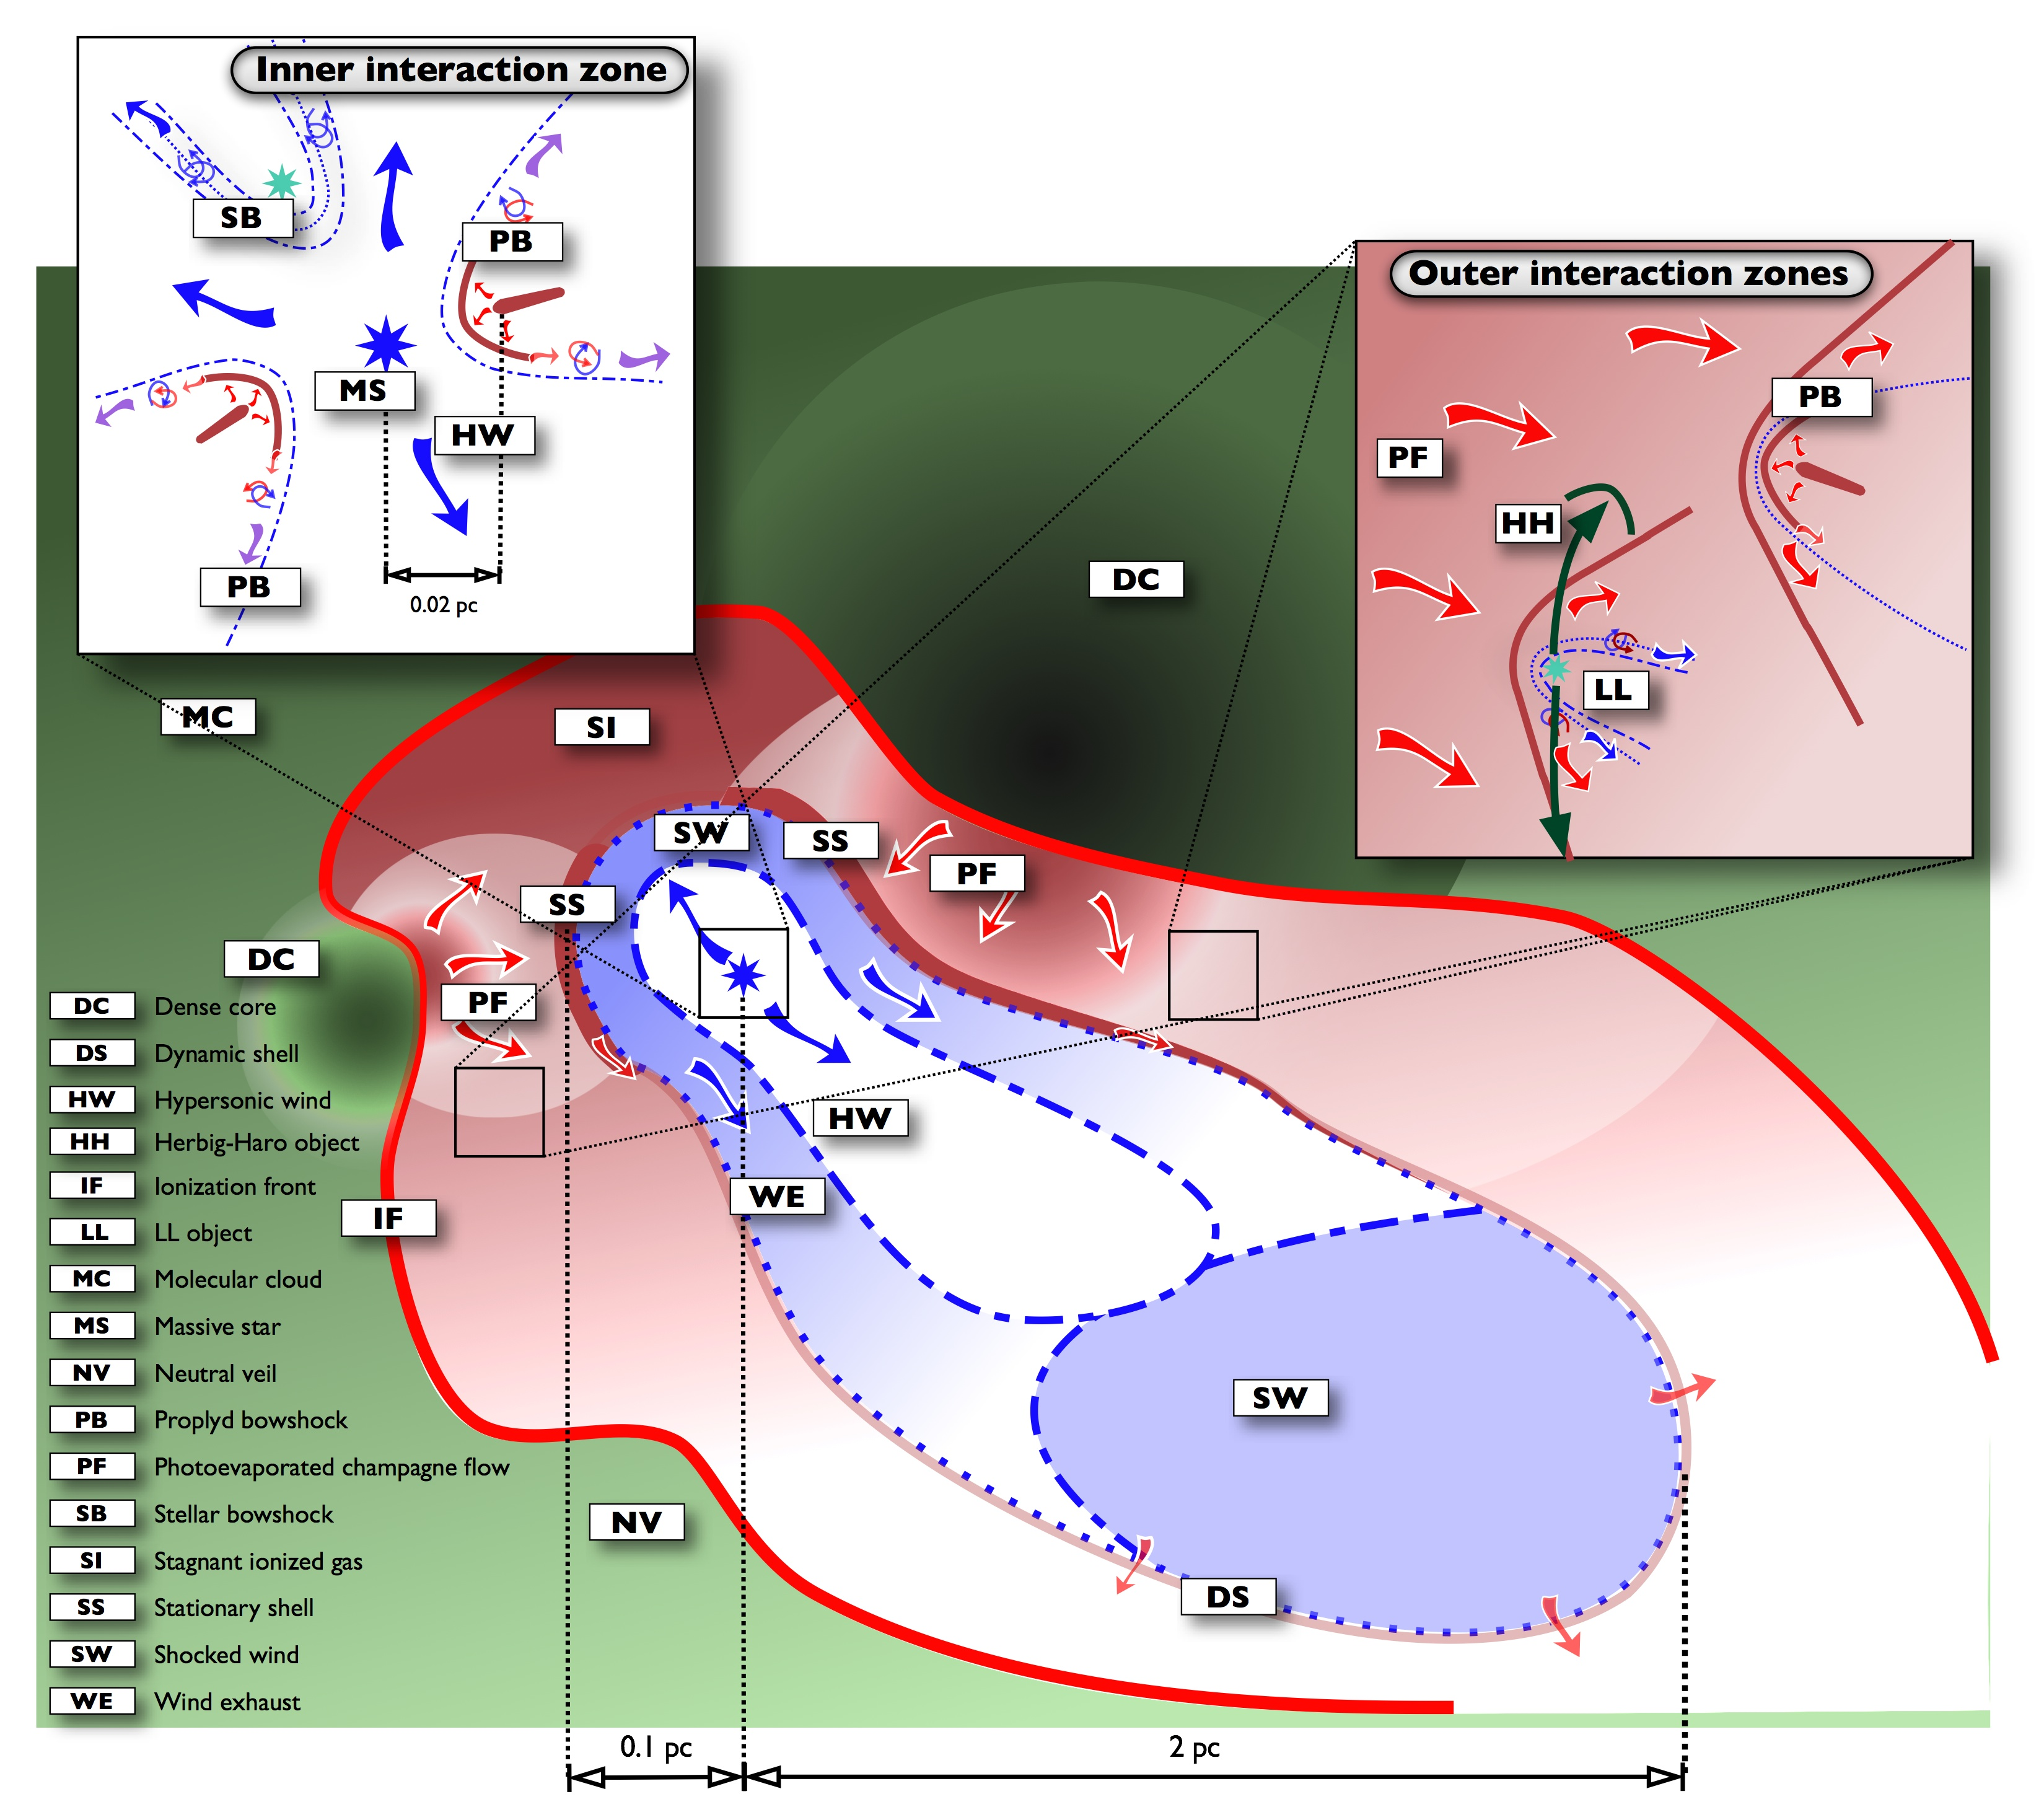
\includegraphics{puebla-figs/wind-geometry-extended}
    \column{0.35\textwidth}
    \Ref{Tarango Yong \& Henney (2016)}\\
    \includegraphics{generic-bowshock}
  \end{columns}
\end{frame}



\begin{frame}
  \frametitle{Positions \& orientations of the bow shocks}
  \centering
  \includegraphics<1>{ll-pos-image}
  \includegraphics<2>{ll-pos-image-zoom}
\end{frame}

\begin{frame}
  \frametitle{Logarithmic spirals in Orion!}
  \begin{columns}
    \column{0.4\textwidth}
    \includegraphics{arc-classify}\\
    \bigskip
    Bow shocks and bright bars form complementary spirals
    \column{0.6\textwidth}
    \includegraphics{spiral-bars}
  \end{columns}
\end{frame}

\begin{frame}
  \frametitle{Speculative 3D structure}
  \includegraphics{orion-3d-twin-view}
\end{frame}

\section{Where should Cloudy fit in?}

\subsection{Macrophysics versus microphysics}

\begin{frame}
  \frametitle{Two complementary approaches to ISM physics}
  \begin{columns}
    \column{0.5\linewidth}\centering
    Team dynamics\\
    \includegraphics{konstandin-turbulent-density-B}\\
    \Ref{Konstandin et al.\ (2015)}
    \column{0.5\linewidth}\centering
    Team microphysics\\
    \includegraphics{o2-grotrian}\\
    \Ref{Moore \& Merril (1968)}
  \end{columns}
  \begin{tikzpicture}
    \draw<2> (current page.center) node[fill=white!50!yellow!90!black, text
    width=0.75\textwidth, opacity=0.9, yshift=-20pt]
    {%
      \vspace*{-\medskipamount}
      \begin{block}{Conservation equations}
        \begin{align*}
          \frac{\partial n_i}{\partial t} + \VEC{\grad} \cdot \bigl( n_i \VEC{u} \bigr)
          & = \sum_{j \ne i} R_{j \to i} n_j  - n_i \sum_{j \ne i} R_{i \to j} \\
          \text{evolution} + \text{div flux}
          & = \text{sources} - \text{sinks}
        \end{align*}
        \textit{\textbf{We need both sides of the equation!}}
        \smallskip
      \end{block}
    };
  \end{tikzpicture}
  
  % \begin{tikzpicture}
  %   \draw (current page.south) [above right=12pt, text width=0.5\textwidth, fill=white]
  %   {hello};
  % \end{tikzpicture}
    % };
\end{frame}

\subsection{Expand microphysics codes to include dynamics}

\begin{frame}
  \frametitle{Non-equilibrium shock models for WR nebulae}
  \centering
  \Ref{Arthur \& Henney, in prep}\\
  \includegraphics{wr-multi-shock-coolcurve}
\end{frame}



\subsection{Improve microphysics in hydro codes}

\begin{frame}
  \frametitle{Weak shocks \(\to\) temperature fluctuations?}
  \centering\includegraphics{diss-plus-ff-t30-th60-ph60}
\end{frame}

\end{document}

%%% Local Variables:
%%% mode: latex
%%% TeX-master: t
%%% End:
